\chapter{Introduction to Deep Learning}

(Revise introduction to instead start by introducing some popular deep learning programs like ChatGPT and search engines, to then delve into neural nets that drive them)

Artificial intelligence is the start to outsourcing brain function to man-made machines.  A machine is said to have "Artificial Intelligence" if it can do what people say requires intelligence \cite{jackson2019introduction}, from counting monetary denominations to surveying Mars, playing chess games to converting human speech.  Within the realm of this is the subcategory known as machine learning, in which models are tested based on training data in order to "teach" them right from wrong.  Machine learning has an increased emphasis on the use of computers in statistical analyses and a decreased emphasis on proving confidence intervals around them \cite{Goodfellow-et-al-2016}.  With astronomical advances in modern computing technology, creating elaborate learning models with raised functionality has become more and more accessible, creating a new category known as deep learning, which is the parent of the subjects within this thesis.  Deep learning models operate beyond those of traditional machine learning as such models contain layers of complexities, each performing a specific task for the overall objective.  Algorithms and procedures unite with complex mathematical formulas to generate extremely precise models without the assumptions of linear models.

%---EXAMPLE FOR PHOTOS--
%--- https://www.overleaf.com/learn/latex/Inserting_Images ---for reference
%\begin{figure}[h]
%    \centering
%    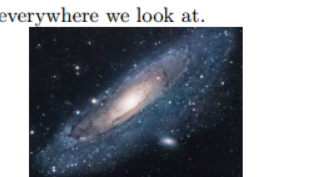
\includegraphics[width=0.25\textwidth]{poo}
%    \caption{a nice plot}
%    \label{fig:mesh1}
%\end{figure}


\section{Overview} %-------------SECTION

Deep learning is the brand of machine learning concerned with using Artificial Neural Networks (ANN's) to reveal complex abstractions within data.
The evolution of the process of mimicking cognitive brain functionality within artificial machines dates back to the 1940's under the term cybernetics, which was originally intended to provide computational models for biological understanding \cite{Goodfellow-et-al-2016}.  Since then, the history of what we now call ``deep learning'' has undergone waves of renaissance.

\subsection{Working with Structured Data} %-------------SECTION

(Regression and Classification tasks, including outlier detection and missing value imputation)

\subsection{Working with Unstructured Data} %-------------SECTION

(Computer vision tasks)

A common elementary application is to utilize a network to recognize and classify image date based on the pixel values, as is shown in Figure \ref{minecraft}.  In image data, each pixel is an input value determined by a number corresponding to that specific color.  For grayscale image data, that number is a value from 0 to 1.  Color images are represented as vectors of three values (RGB).

\begin{figure}[H]
    \centering
%\raisebox{20pt}
    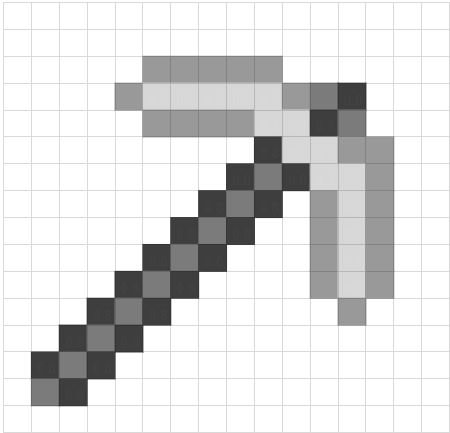
\includegraphics[width=.2\textwidth]{Figures/pickaxe_1.png}
    \hspace{60pt}
    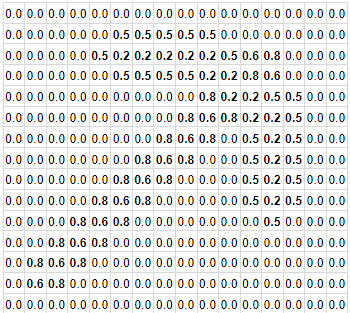
\includegraphics[width=.5\textwidth]{Figures/pickaxe_2.png}
    \caption{\footnotesize{An 16x16 pixel image, with its numerical counterpart next to it.  In greyscale image data, a value of 0.0 corresponds to white, 1.0 to black, and ordered variations of gray to values in between}}
    \label{minecraft}
\end{figure}

Of course, image data is not the only data that a neural network can be used on.  Any type of data can be modeled with a neural network, provided there is enough of it to match the complexity if the model.  Image data tends to have a great number of inputs to begin with.